\documentclass{sigkddExp}
\usepackage{graphicx, caption, subcaption}
%%%%%%%%%%%%%%%%%%%%%%%%%%%%%%%%%%%%%%%%%%%%%%%%%%%%%%%%%%
% TITLE
%%%%%%%%%%%%%%%%%%%%%%%%%%%%%%%%%%%%%%%%%%%%%%%%%%%%%%%%%%
%Title will probably change
\title{[PAPER DROP 1]\\
Predicting crime rates using taxi rides data}


%%%%%%%%%%%%%%%%%%%%%%%%%%%%%%%%%%%%%%%%%%%%%%%%%%%%%%%%%%
% AUTHORS
%%%%%%%%%%%%%%%%%%%%%%%%%%%%%%%%%%%%%%%%%%%%%%%%%%%%%%%%%%
\numberofauthors{3}
\author{
\alignauthor Carlos Petricioli \\
       % \affaddr{Computer Science Department}\\
       \affaddr{New York University}\\
       \affaddr{New York, USA}\\
       \email{petricioli@nyu.edu}
\alignauthor Valerie Angulo\\
       % \affaddr{Computer Science Department}\\
       \affaddr{New York University}\\
       \affaddr{New York, USA}\\
       \email{vaa238@nyu.edu}
\alignauthor Varsha Muralidharan \\
       % \affaddr{Computer Science Department}\\
       \affaddr{New York University}\\
       \affaddr{New York, USA}\\
       \email{vm1370@nyu.edu}
}


\begin{document}

\maketitle

%%%%%%%%%%%%%%%%%%%%%%%%%%%%%%%%%%%%%%%%%%%%%%%%%%%%%%%%%%
% ABSTRACT
%%%%%%%%%%%%%%%%%%%%%%%%%%%%%%%%%%%%%%%%%%%%%%%%%%%%%%%%%%
\begin{abstract}

Understanding and predicting crime is a crucial task in any major city. The objective of this study is to understand crime rates and its effects on how the use of taxis in New York City at a granular level. The idea  is that people react according to how secure they feel, which extends to their travel preferences. 
Our hypothesis is that people are less likely to walk in areas subjectively deemed more dangerous, and will instead opt to use more reliable and immediate transportation such as designated taxis. 
New York City will be used in this study as it provides a large amount of public data on crimes throughout the five boroughs along with an extensive amount of data from NYC yellow cab usage. 
This approach that will complement the use of demographics and geographical variables commonly used to predict crime. Global Positioning System (GPS) data on taxi rides provide useful information that can be directly related to crime. Also, weather data will be used as a control factor which might have a direct impact on people's taxi usage. 

\end{abstract}



%%%%%%%%%%%%%%%%%%%%%%%%%%%%%%%%%%%%%%%%%%%%%%%%%%%%%%%%%%
% INTRODUCTION
%%%%%%%%%%%%%%%%%%%%%%%%%%%%%%%%%%%%%%%%%%%%%%%%%%%%%%%%%%

\section{Motivation}

Understanding and predicting crime is a crucial task in any major city. 
The ability to understand criminal activity in a very delimited area adds depth to the current understanding of crime and  it provides a baseline to understand its effect on people's behavior. 
This question is relevant because it has a direct impact on the families economies since taking a taxi is the most expensive public transportation option and might also have an impact on people's health because there might be avoiding to walk to avoid crime which directly reduces peoples physical activity and might impact their health in the long run. 
This fact could translate into a much bigger public health issue for the city in the long run. %%% A LOT OF CITES NEEDED HERE.

Specifically, we picked New York City because it has the largest  total number of offenses known to law enforcement by city crime according to the FBI's Uniform Crime Reporting \cite{fbiUniformCrime}, with a total of around 223 thousand for 2016 over cities like Los Angeles, Houston and Chicago, which have 156, 148 and
147 thousand offenses respectively. 
This provides the most vast crime dataset for this analysis.
Also, New York City has an Open Data Law which mandates that all public crime data be available online \cite{OpenDat}, which makes crime data collection easily accessible to the public.


% Our primary reason is thatThere are an abundance of transportation services available in New York City and taxi data is common enough to garner a big data set. 
%THIS IS NOT THEEEE PRIAMARY REASON ITS JUST CONVENIENT FOR US. THE PRIMARY REASON SHOULD BE THAT WE CONSIDER NYC INTERESTING FOR ITS BLAAA..., IT COULD BE ANYTHING BUT THERE ARE ABUNDANCE OF TRANSPORTANTION SERVICES IN MANY PLACES AND WE STILL PICKED NYC BECAUSE X.


% IN NOT SURE THIS IS ACUTALLY TRUE IF IT IS WE SHOULD CITE SOMETHING: 
       % It is also easy for individuals to choose a reliable taxi company, the NYC yellow taxi, which is a widely used and reputable taxi company. 
% With the abundance of transportation options, our study can explore transportation patterns such as taxi usage versus subway usage based on subway locations and taxi pickup/drop off coordinates. %ITS NOT VS SUBWAY USAGE BECASE WE CANNOT BE SURE OF THAT. IT SHOULD BE SOMETHING LIKE TAXI USAGE GIVEN THE PROXIMITY TO A SUBWAY STATION AT A GIVEN LOCATION.
\section{Introduction}

It is hard to argue that violence and crime is not a relevant factor that people take into consideration when commuting among the boroughs of New York city. 
So, this work assumes that that people want to minimize the time spent in locations they consider unsafe which  plays a roll in their transportation preferences affecting their taxi usage. 

What goes into an individuals subjective view of what is safe versus unsafe can be hard to gage. However, a lot can be inferred from an individuals behavior patterns.
One such pattern of behavior is transportation habits. The idea is to correlate taxi pickup and drop off information to the perceived level of crime activity in an area. 
It is inferred that people choose to not use public modes of transportation in areas where an individual feels unsafe or uncomfortable and will instead opt to use a more direct and safer source such as a designated taxi. 
% Through open source data of taxi trips, we hope to correlate peoples transportation behavior with the rate of crime activity in a given area. 



% Relating crime to transportation is important because it uses the knowledge of those who live in an area to predict which areas may be more prevalent to crime. %I DONT LIKE THIS SENTENCE HAHA. 
% This is an intuitive source of information that utilizes people and their knowledge of the city in crime prediction. %SAME HERE THIS IS A COMPLEX THING TO SAY WE SHOULD KEEP IT SIMPLE 

This study can give a look into what areas people avoid, allowing to geographically match the locations of crime activity to geographical pickup/drop off locations of taxi trips provided in the open source taxi data and can also provide information into the development of areas that become more or less crime ridden. 

To perform all the analysis, three main datasets were chosen.
The Taxi \& Limousine Commission (TLC) provide open data for all the rides in New York City since 2009 up to the present \cite{Taxi}. 
The crime data collected for this study contains historic \cite{NYPDHis} and current \cite{NYPDCur} records from NYPD complaint data, which has crimes reported since 2006 until present.
Data collected from the National Oceanic and Atmospheric Administration (NOAA) \cite{NOAA} is used as a third data source in order to provide a more controlled analysis. Specifically, hourly weather data  captured from three stations, Central Park, JFK airport, and La Guardia airport stations, is used as a possible explanation for taxi/crime patterns that do not correlate, seeing as weather is often a factor in the decision to take certain forms of transportation.

%NOT ACCURATE NOT HERE: For this study, we will compare the distance of taxi pickup locations to reported locations of crime activity. This is so that we can unite these two data sources based on geographic locations within the city. 

These three data sets were downloaded into a Hadoop cluster\footnote{NYU's High Perfomance Computing Hadoop cluster, Dumbo}, as shown in Figure \ref{figx}. Both crime and taxi data contain latitude and longitude data, which provide a very granular way of relating the datasets. 
This was achieved by a spatial join formulated as a Map/Reduce problem in order to exploit the benefits of the cluster. 
The problem was, how to join the  longitude and latitude coordinates for crime activity with the coordinates for taxi usage to a specific area  in New York City   in order to have a commonly defined location between the two sources.
Also, hourly weather data collected at three points, Central Park, LaGuardia and JFK, was assigned to each taxi ride by picking the data collected from the nearest station to the pickup location at a given time. 




%%%%%%%%%%%%%%%%%%%%%%%%%%%%%%%%%%%%%%%%%%%%%%%%%%%%%%%%%%
% RELATED WORK
%%%%%%%%%%%%%%%%%%%%%%%%%%%%%%%%%%%%%%%%%%%%%%%%%%%%%%%%%%

%%% THIS HAS TO BE MUCH MORE DETAILED
\section{Related Work}

There have been some studies on big data sources used in conjunction with crime data in order to understand and predict crime patterns. 
In one such study \cite{Wang16}, the authors propose to complement the traditional ways of predicting crime rates by including the use points of interest (POI) and taxi flow data in Chicago. 
In that study, it is hypothesized that taxi flows are ``hyper links'' within a city that connect locations, where they may be a proxy for broader patterns of population routine activity and mobility, commuting flows, and other forms of social and economic exchanges between two communities over space. The authors use POI to enhance the demographics information and use taxi flow as hyper links to enhance the geographical proximity correlation however, the temporal dimension of crime is not considered in depth. The problem in this study is population-centric, where the crime rate for Chicago is profiled in community areas that are well-defined and stable geographical regions. The proposed POI features and taxi links provide new perspectives in profiling the crime rate across community areas and the crime data collected in Chicago contains detailed information about the time, location and type of crime committed.

Other studies utilize crowd sourced data to predict crime patterns. In a recent study \cite{Bendler14} crowd sourcing of tweets was used as a virtual neighborhood watch in order to find crime patterns. The rough location for where the twitter post was sent can be determined by the social network provider or by geo-tags from the users phone. This study inferred that there was a correlation between an important event and the amount of tweets traced to a specific area, where an increase in the amount of tweets in a given area within a certain time span suggests an event was occurring at that time and place. The goal of this study was to predict and explain crimes in urban areas through tweet volume where crime and tweets were related through time and location. This study collected tweets and crime data in hourly blocks at Market Street in San Fransisco during a duration of three months. 

Urban crime has been correlated with different modes of communication data as well. The authors of a recent study \cite{Traunmueller14} presented a method to relate crime in London and people dynamics through the utilization of crime data records for the area of Greater London and data from a mobile telecommunication provider for details of people dynamics. Crime data was recorded with latitude/longitude coordinates whereas the telecommunication data was available as footfall in grids of varying sizes (smaller grids in central London as opposed to larger grids in less densely populated areas outside central London). While many people dynamics were looked at in depth in regards to crime, there were two major limitations in the study performed. One was that the crime data was recorded on a monthly basis whereas the telecommunications data recorded footfall on an hourly basis. This limitation is avoided in our study by grouping the data together by hour so that it is more cohesive. Because our study emphasizes time and location of taxi usage, crime activity and surrounding weather conditions, we have made sure that our three data sources share these conditions.


\section{Design}

Figure \ref{figx} shows our data flow diagram\footnote{DUMBO refers to NYU's High Performance Computing Hadoop cluster}.  It shows that all three data sources were downloaded into a Hadoop cluster and cleaned in spark and later stored as Spark's SQL tables which can be read as Hive or Impala tables.

\begin{figure}
\caption{Data flow diagram}
\label{figx}
\centering 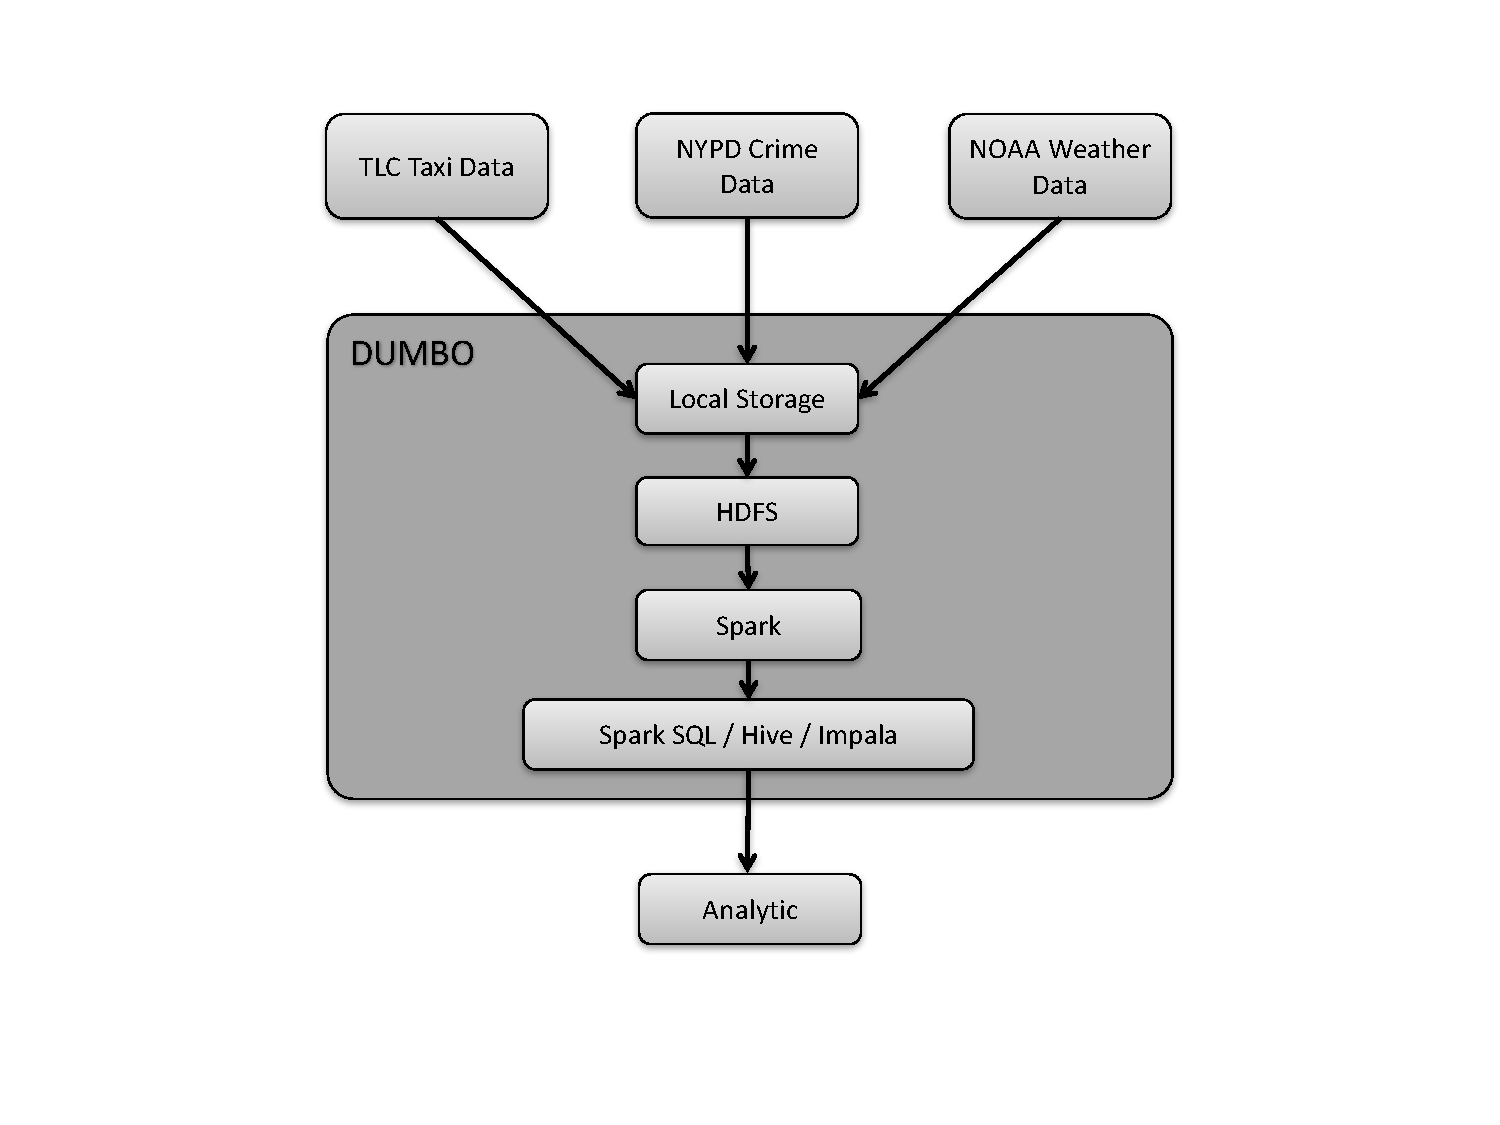
\includegraphics[width=.45\textwidth]{images/DesignFlowDiagram.pdf}
\end{figure}


\subsection{Getting and cleaning the data}

Getting the data was fairly easy because all three sets have APIs which provide a reliable and easy access.

\subsubsection{Crimes data}
There were a few anomalies that were found in the NYPD crime datasets. The two datasets (historic and current crime) at hand were for crimes that were reported from 2006 till present. However, certain records had incorrect or bad entries in the Crime Start and End Date-Time columns. For instance, there were several crimes reported to have occurred in the year 1016, which were assumed as a typological error for the year 2016. These records were fixed and used in the analytic. A few other records with year entries such as 1026 were dropped, as appropriate inferences could not be drawn. Certain records\footnote{Which make us wonder how much should we trust this dataset, but, still, it is what we have.} had timestamps of \texttt{24:00:00}, and were corrected to \texttt{00:00:00}.

\subsubsection{TLC data}
As expected there were complications while cleaning the Taxi rides data from TLC.

\subsection{Description of the data}


\subsection{Analytic}

Crime occurrences will be divided into  two levels: \textit{high crime} and  \textit{low crime} with respect to the total number of observed number crimes in a given period of time which will be defined later.
So crime level can be defined at every time $t$ an location $l$ as a binary variable for \textit{high crime} and \textit{low crime} when the total number of crime at is respectively higher and lower  than the average for that time and location.

To simplify things, any location is considered to have a  distance to a subway entrance equal to 0 if the location has any number available subway entrances,  1 if any of its neighbors location has a distance of 0 and 2 in every other case. \textbf{NOTE:} This assumption will be revised later to mark differences when a location has a lot vs just one entrance because it is important while making a very granular analysis.


Any taxi ride will be categorized as a \textit{short ride} if the distance form the pickup location to drop off location is considered as: could be walked in in less than a given time (i.e. 10 minutes) for an average person. And \textit{long ride} any other case.

With this implementation we  can to answer this type of questions:
\begin{enumerate}
       \item Is the average number of taxi pickups different in areas that have different levels of crime rates?

       \item Is the average number of taxi pickups different in areas that have different levels of crime rates grouping by the proximity of an area to a \textbf{subway}? 

       \item Is the average number of taxi pickups different in areas that have different levels of crime rates when we compare at times with and without \textbf{rain} (or different weather variables)?

       \item Does the average  number of \textbf{short} rides hve a different average number of taxi pickups  in areas that have different levels of crime rates  compared to the average of \textbf{long} rides?

       \item Does the answer of the previous questions change for special dates such as \textbf{holidays}?

       \item When categorized by the \textbf{severity of crime}, is the average number of taxi pickups different in areas that have different levels of crime rates for a given level of severity in crimes?

       \item \textbf{Run away vs feel attracted} to crime. When there are ``high profiled'' crime incidents in a given location does the average number of drop offs is greater, lower or similar to the average?\footnote{\textbf{NOTE:} This is a similar question to \cite{Bendler14}.}

       \item Given crime rates changes across time for a given area, is the average number of taxi pickups  changing too? If so, same direction? With a time lag?
       does it lasts long? Does severity has an impact?

       \item How does the error in the prediction of crime rates changes when modeling it with traditional demographics vs the taxi rides vs both as features?\footnote{
       \textbf{NOTE:} This is the main question of the paper from KDD 2016 \cite{Wang16}. }

\end{enumerate}


\begin{figure}
\label{fig:zones}
    \centering
    \begin{subfigure}[t]{0.25\textwidth}
        \centering
        \label{fig:zones_shape}
        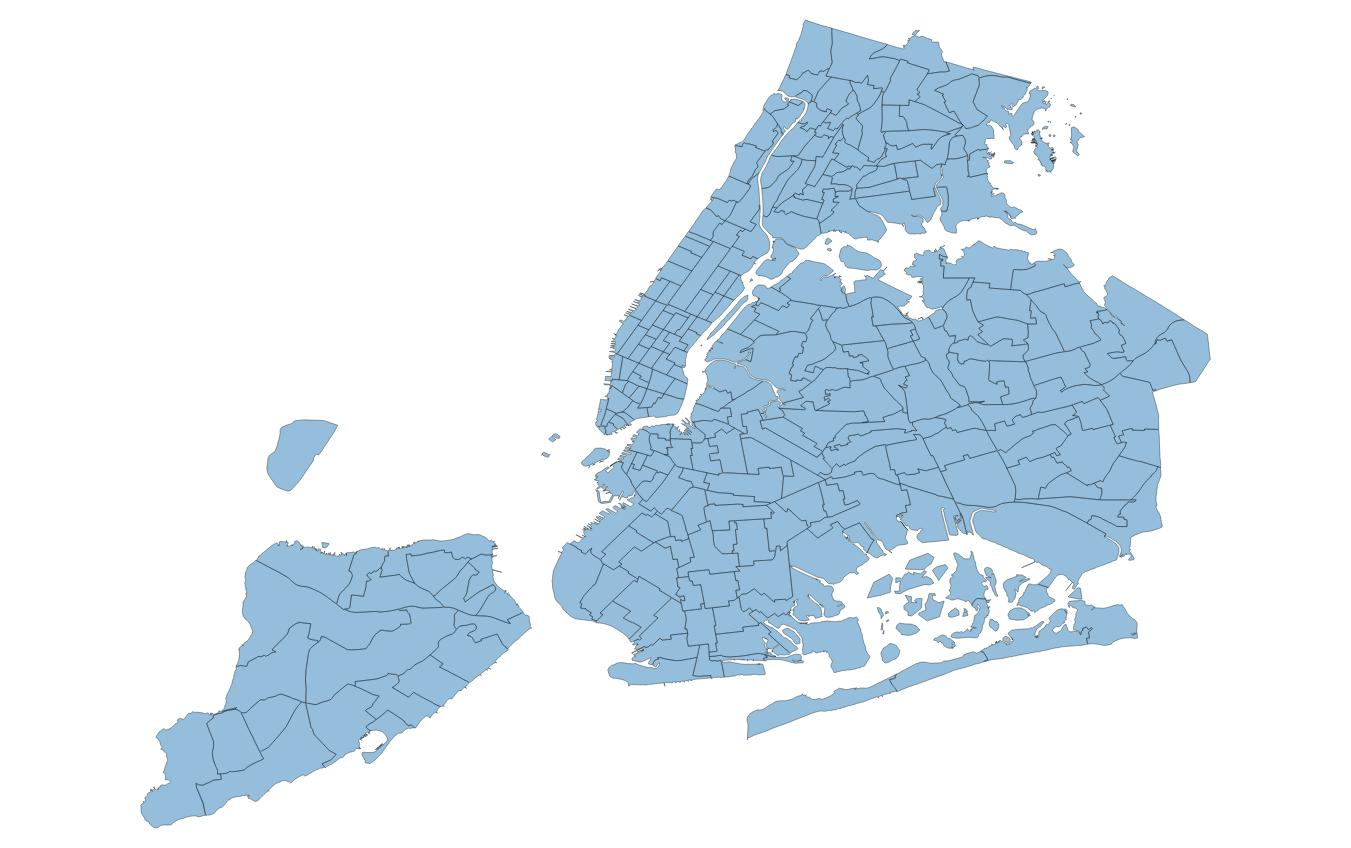
\includegraphics[height=1.2in]{images/taxi_zones_shape}
        \caption{Shape}
    \end{subfigure}%
    ~ 
    \begin{subfigure}[t]{0.25\textwidth}
        \centering
        \label{fig:zones_raster}
        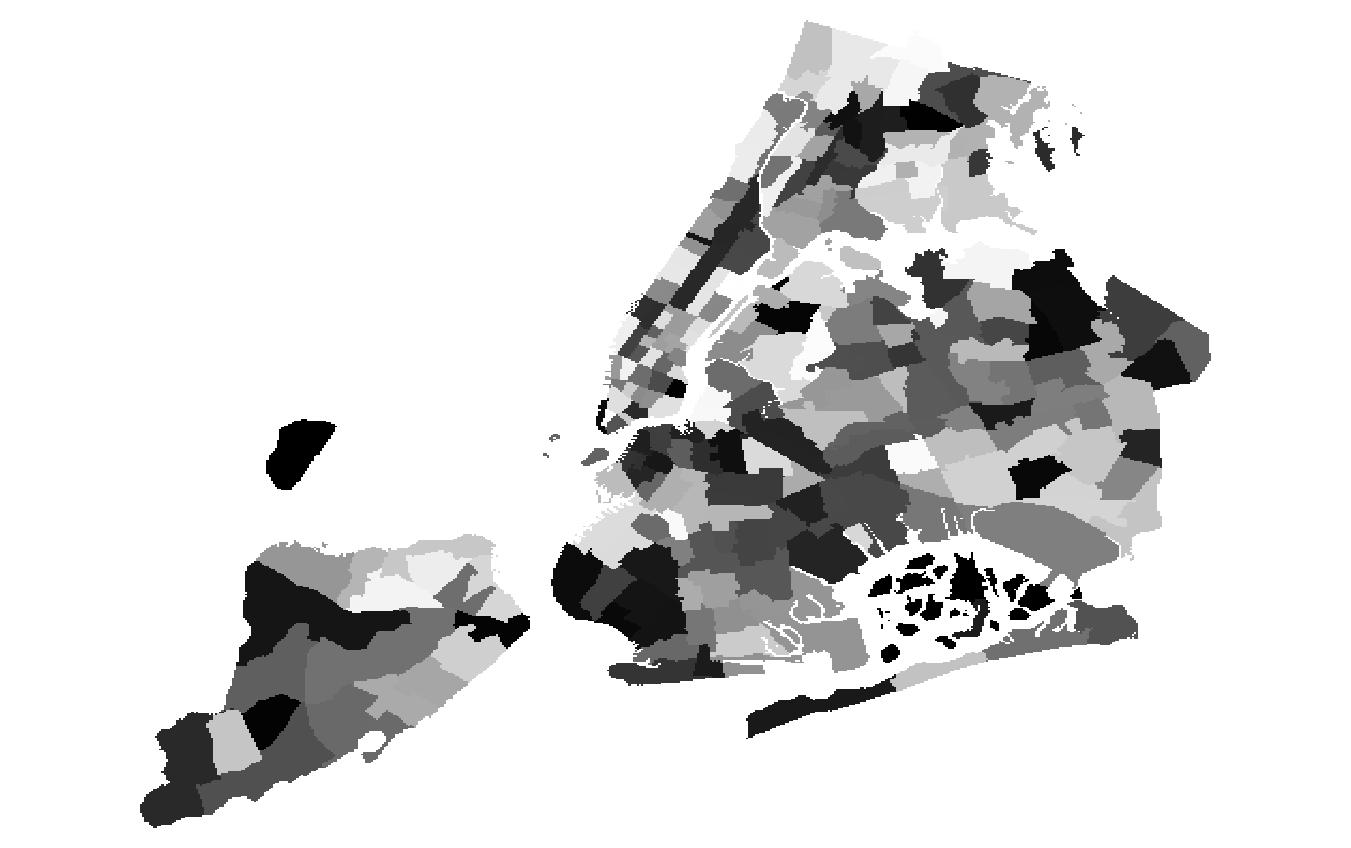
\includegraphics[height=1.2in]{images/taxi_zones_raster}
        \caption{Raster}
    \end{subfigure}
    ~ 
    \begin{subfigure}[t]{0.5\textwidth}
        \centering
        \label{fig:zones_both}
        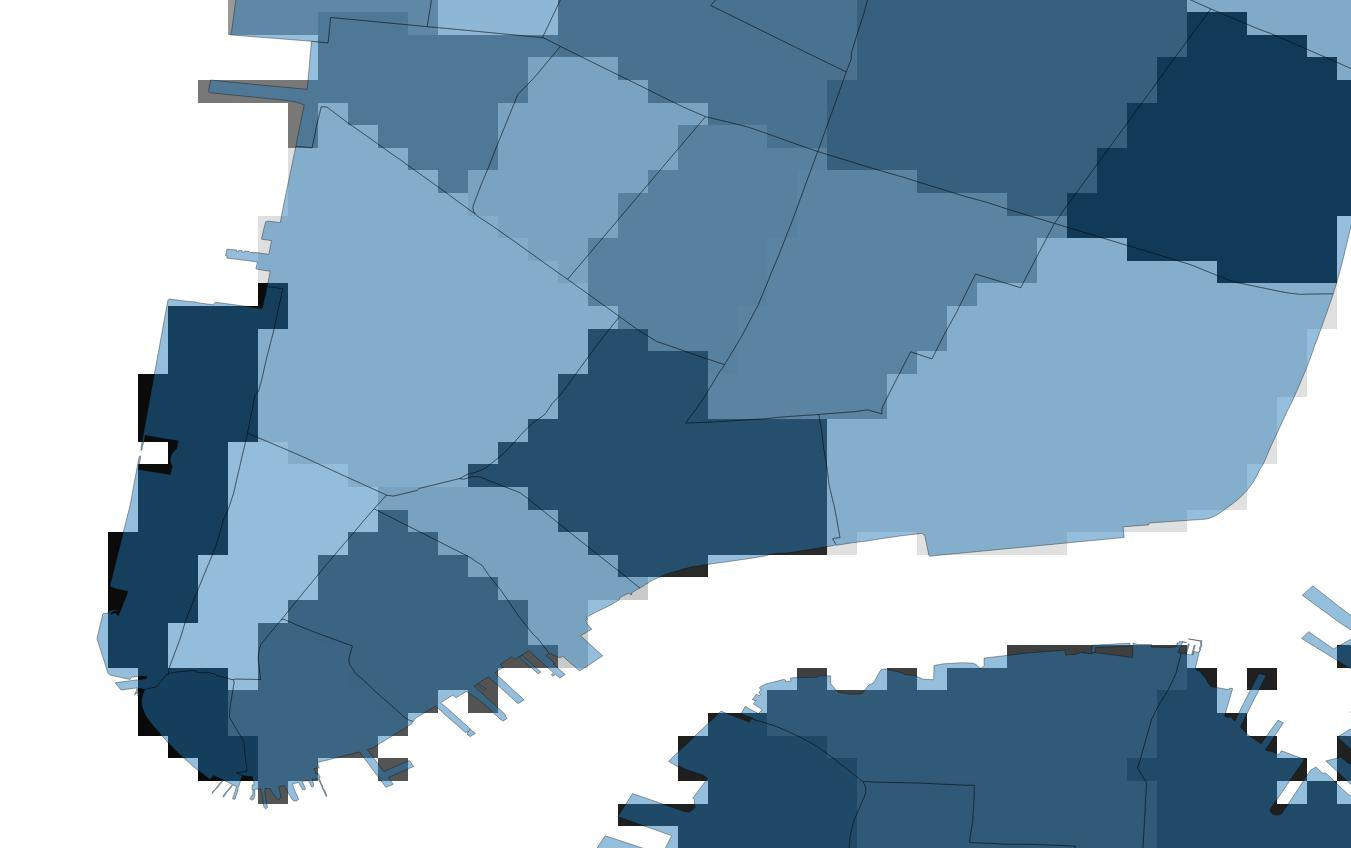
\includegraphics[width=0.5\textwidth]{images/both}
        \caption{Both}
    \end{subfigure}
    \caption{NYC Taxi zones file formats}
\end{figure}


\section{Limitations}
Our proposed method to quantitatively study crime rates in the city of New York intends to test the appropriateness of employing New York City TLC data and NOAA weather data as a suitable indicator for criminal activity in different New York City neighborhoods. Although the results of our study produce a considerable degree of validity, our work suffers from a few limitations. 
In the age of app-based transportation technology, companies such as Uber and Lyft are challenging the age-old taxi industry. 
A significant portion of the city's population makes use of these options over New York City taxis because of numerous reasons. 
For one, Uber's new strategy of making their services more available in the outer boroughs of New York City where taxis are scarce and access to public transport is not easy. Nevertheless, the TLC industry is still strong and serves roughly 50\% of city-wide taxi users.
%%%%%%%%%%%%%%%%%%%%%%%%%%%%%%%%%%%%%%%%%%%%% 
%%CITATION NEADED HEEERE for percentage of taxi usage
%%%%%%%%%%%%%%%%%%%%%%%%%%%%%%%%%%%%%%%%%%%


%%%%%%%%%%%%%%%%%%%%%%%%%%%%%%%%%%%%%%%%%%%%%%%%%%%%%%%%%%
% CONCLUSIONS
%%%%%%%%%%%%%%%%%%%%%%%%%%%%%%%%%%%%%%%%%%%%%%%%%%%%%%%%%%

% \section{Conclusions}
% This paragraph will end the body of this sample document.
% Remember that you might still have Acknowledgements or
% Appendices; brief samples of these
% follow.  There is still the Bibliography to deal with; and
% we will make a disclaimer about that here: with the exception
% of the reference to the \LaTeX\ book, the citations in
% this paper are to articles which have nothing to
% do with the present subject and are used as
% examples only.
%\end{document}  % This is where a 'short' article might terminate



%%%%%%%%%%%%%%%%%%%%%%%%%%%%%%%%%%%%%%%%%%%%%%%%%%%%%%%%%%
%ACKNOWLEDGEMENTS are optional
%%%%%%%%%%%%%%%%%%%%%%%%%%%%%%%%%%%%%%%%%%%%%%%%%%%%%%%%%%
% \section{Acknowledgments}
% This section is optional; it is a location for you
% to acknowledge grants, funding, editing assistance and
% what have you.  In the present case, for example, the
% authors would like to thank Gerald Murray of ACM for
% his help in codifying this \textit{Author's Guide}
% and the \textbf{.cls} and \textbf{.tex} files that it describes.



%%%%%%%%%%%%%%%%%%%%%%%%%%%%%%%%%%%%%%%%%%%%%%%%%%%%%%%%%%
% REFERENCES
%%%%%%%%%%%%%%%%%%%%%%%%%%%%%%%%%%%%%%%%%%%%%%%%%%%%%%%%%%
% ACM needs 'a single self-contained file'! SO WE'll NEED TO CHANGE THIS AT THE END.
\bibliographystyle{abbrv}
\bibliography{biblio} 



%%%%%%%%%%%%%%%%%%%%%%%%%%%%%%%%%%%%%%%%%%%%%%%%%%%%%%%%%%
% APPENDIX
%%%%%%%%%%%%%%%%%%%%%%%%%%%%%%%%%%%%%%%%%%%%%%%%%%%%%%%%%%
%APPENDICES are optional
% \balancecolumns
% \appendix
% %Appendix A
% \section{Headings in Appendices}


\end{document}
